\documentclass[25pt,a0paper,landscape]{tikzposter}
\usetheme{Board}
\usepackage[utf8]{inputenc}
\usepackage{xurl}
% \usepackage{natbib}
\usepackage{amsmath,amssymb}
\usepackage{pstricks}
\usepackage{pst-barcode}
% \usepackage{iftex}
\usepackage{textcomp} % provide euro and other symbols
% \usepackage{lmodern}
% % Use upquote if available, for straight quotes in verbatim environments
% \IfFileExists{upquote.sty}{\usepackage{upquote}}{}
% \IfFileExists{microtype.sty}{% use microtype if available
%   \usepackage[]{microtype}
%   \UseMicrotypeSet[protrusion]{basicmath} % disable protrusion for tt fonts
% }{}
% \makeatletter
% \@ifundefined{KOMAClassName}{% if non-KOMA class
%   \IfFileExists{parskip.sty}{%
%     \usepackage{parskip}
%   }{% else
%     \setlength{\parindent}{0pt}
%     \setlength{\parskip}{6pt plus 2pt minus 1pt}}
% }{% if KOMA class
%   \KOMAoptions{parskip=half}}
% \makeatother
\usepackage{xcolor}
% Define solarized colors
\definecolor{solarized-base03}{HTML}{002b36}
\definecolor{solarized-base02}{HTML}{073642}
\definecolor{solarized-base01}{HTML}{586e75}
\definecolor{solarized-base00}{HTML}{657b83}
\definecolor{solarized-base1}{HTML}{839496}
\definecolor{solarized-base2}{HTML}{93a1a1}
\definecolor{solarized-base3}{HTML}{e7e9db}
\definecolor{solarized-yellow}{HTML}{b58900}
\definecolor{solarized-orange}{HTML}{cb4b16}
\definecolor{solarized-red}{HTML}{dc322f}
\definecolor{solarized-magenta}{HTML}{d33682}
\definecolor{solarized-violet}{HTML}{6c71c4}
\definecolor{solarized-blue}{HTML}{268bd2}
\definecolor{solarized-cyan}{HTML}{2aa198}
\definecolor{solarized-green}{HTML}{859900}

\setlength{\emergencystretch}{3em} % prevent overfull lines
\providecommand{\tightlist}{%
  \setlength{\itemsep}{0pt}\setlength{\parskip}{0pt}}
\setcounter{secnumdepth}{-\maxdimen} % remove section numbering
\usepackage{tikz}
\usepackage{tikz-cd}
\usepackage[most]{tcolorbox}
\usetikzlibrary{decorations.pathmorphing,shadows.blur,shadings}
\tcbuselibrary{skins}
%\pgfmathsetseed{1} % To have predictable results

% Define a background layer, in which the parchment shape is drawn
% \pgfdeclarelayer{background}
% \pgfsetlayers{background,main}

% This is the base for the fractal decoration. It takes a random point
% between the start and end, and raises it a random amount, thus
% transforming a segment into two, connected at that raised point This
% decoration can be applied again to each one of the resulting
% segments and so on, in a similar way of a Koch snowflake.
\pgfdeclaredecoration{irregular fractal line}{init}
{
  \state{init}[width=\pgfdecoratedinputsegmentremainingdistance]
  {
    \pgfpathlineto{%
      \pgfpoint{random * \pgfdecoratedinputsegmentremainingdistance}{%
        (random * \pgfdecorationsegmentamplitude - 0.02) *
         \pgfdecoratedinputsegmentremainingdistance}}
    \pgfpathlineto{\pgfpoint{\pgfdecoratedinputsegmentremainingdistance}{0pt}}
  }
}

% Define paper style
\tikzset{
  paper/.style={%
    draw=black!10,
    blur shadow,
    path picture={%
      \fill[solarized-base3!50!white] ([shift={(-5pt,-5pt)}]path picture bounding box.south west) rectangle ([shift={(5pt,5pt)}]path picture bounding box.north east);
    }
  },
  irregular border/.style={%
    decoration={irregular fractal line, amplitude=0.2},
    decorate,
  },
  ragged border/.style={%
    decoration={random steps, segment length=7mm, amplitude=2mm},
    decorate,
  }
}

\newtcolorbox{quotebox}{%
  % enhanced jigsaw, <-- Beware, This rendering engine let the
  %                      frame appear on some PDF viewers
  empty, % Better use this rendering engine to avoid the bug
  interior code={%
    % \begin{pgfonlayer}{background}  % Draw the shape behind
      \fill[paper] % recursively decorate the bottom border
      decorate[irregular border]{%
        decorate{decorate{decorate{decorate[ragged border]{
                ($(interior.south east) - (0, random * 5mm)$) --
                ($(interior.south west) - (0, random * 5mm)$)
              }
            }
          }
        }
      }
      -- (interior.north west) -- (interior.north east) -- cycle;
    % \end{pgfonlayer}
  },
  sharp corners,
  boxrule=0pt,
  left=5pt,
  right=5pt,
  top=5pt,
  bottom=0.5em,
  after skip=10mm,
}

%% TColorBox Note environment
\newlength\savedparindent
\setlength\savedparindent\parindent
\newenvironment{tnote}[1]{%
  \begin{tcbnote}{}
    \setlength\parindent{\savedparindent}
    \begin{center}
      \sffamily\bfseries\LARGE #1
    \end{center}\par
  }{%
  \end{tcbnote}
}
% Color box styles
\newtcolorbox{tldrbox}{
  colback=solarized-blue!5!white,
  colframe=solarized-blue!75!black,
  title=TL;DR,
  enhanced,
  drop shadow southeast,
  boxrule=2pt,
  fonttitle=\bfseries\large,
  sharp corners=south,
  rounded corners=north,
  interior style={top color=solarized-blue!5!white, bottom color=solarized-blue!20!white}, 
}
\newtcolorbox{proofbox}[1][]{
  colback=solarized-cyan!5!white,
  colframe=solarized-cyan!75!black,
  enhanced,
  drop shadow southeast,
  boxrule=2pt,
  sharp corners=south,
  rounded corners=north,
  interior style={top color=solarized-cyan!1!white, bottom color=cyan!5!white}, 
  #1
}
\newtcolorbox{theorybox}[1][]{
  colback=solarized-yellow!5!white,
  colframe=solarized-yellow!75!black,
  enhanced,
  drop shadow southeast,
  boxrule=2pt,
  sharp corners=south,
  rounded corners=north,
  interior style={top color=solarized-yellow!5!white, bottom color=solarized-yellow!10!white}, 
  #1
}
\newtcolorbox{examplebox}[1][]{
  colback=solarized-violet!5!white,
  colframe=solarized-violet!75!black,
  enhanced,
  drop shadow southeast,
  boxrule=2pt,
  sharp corners=south,
  rounded corners=north,
  interior style={top color=solarized-violet!5!white, bottom color=solarized-violet!10!white}, 
  #1
}
\newtcolorbox{backgroundbox}[1][]{
  colback=solarized-base00!5!white,
  colframe=solarized-base00!75!black,
  enhanced,
  drop shadow southeast,
  boxrule=2pt,
  sharp corners=south,
  rounded corners=north,
  interior style={top color=solarized-base00!5!white, bottom color=solarized-base00!10!white}, 
  #1
}


\usepackage{graphicx}
\usepackage{multicol}
\usepackage{amsmath,amsfonts,amssymb,amsthm,bm}
\usepackage{mathtools}
\DeclareMathOperator{\opExpectation}{\mathbb{E}}
\newcommand{\E}[2]{\opExpectation_{#1} \left [ #2 \right ]}
\newcommand{\simpleE}[1]{\opExpectation_{#1}}
\newcommand{\MidSymbol}[1][]{\:#1\:}
\newcommand{\given}{\MidSymbol[\vert]}
\DeclareMathOperator{\opmus}{\mu^*}
\newcommand{\IMof}[1]{\opmus[#1]}
\DeclareMathOperator{\opInformationContent}{H}
\newcommand{\ICof}[1]{\opInformationContent[#1]}
\newcommand{\xICof}[1]{\opInformationContent(#1)}
\DeclareMathOperator{\opEntropy}{H}
\newcommand{\Hof}[1]{\opEntropy[#1]}
\newcommand{\xHof}[1]{\opEntropy(#1)}
\DeclareMathOperator{\opMI}{I}
\newcommand{\MIof}[1]{\opMI[#1]}
\DeclareMathOperator{\opTC}{TC}
\newcommand{\TCof}[1]{\opTC[#1]}
\newcommand{\CrossEntropy}[2]{\opEntropy(#1 \MidSymbol[\Vert] #2)}
\newcommand{\iCrossEntropy}[3]{\opEntropy_{#1 \Vert #2}[#3]}
\DeclareMathOperator{\opKale}{D_\mathrm{KL}}
\newcommand{\Kale}[2]{\opKale(#1 \MidSymbol[\Vert] #2)}
\newcommand{\iKale}[3]{\opKale_{,\, #1 \Vert #2}[#3]}
\DeclareMathOperator{\opJSD}{D_\mathrm{JSD}}
\newcommand{\JSD}[2]{\opJSD(#1 \MidSymbol[\Vert] #2)}
\DeclareMathOperator{\opp}{p}
\newcommand{\pof}[1]{\opp(#1)}
\newcommand{\hpof}[1]{\hat{\opp}(#1)}
\newcommand{\pcof}[2]{\opp_{#1}(#2)}
\newcommand{\hpcof}[2]{\hat\opp_{#1}(#2)}
\DeclareMathOperator{\opq}{q}
\newcommand{\qof}[1]{\opq(#1)}
\newcommand{\hqof}[1]{\hat{\opq}(#1)}
\newcommand{\qcof}[2]{\opq_{#1}(#2)}
\newcommand{\varHof}[2]{\opEntropy_{#1}[#2]}
\newcommand{\xvarHof}[2]{\opEntropy_{#1}(#2)}
\newcommand{\varMIof}[2]{\opMI_{#1}[#2]}
\newcommand{\w}{\boldsymbol{\theta}}
\newcommand{\W}{\boldsymbol{\Theta}}
\newcommand{\h}{\boldsymbol{\phi}}
\newcommand{\hopt}{\boldsymbol{\h^\star}}
\newcommand{\Hyper}{\boldsymbol{\Phi}}
\DeclareMathOperator{\opf}{f}
\newcommand{\fof}[1]{\opf(#1)}
\newcommand{\xset}[3]{(\x_n^{#1})_{n=#2}^{#3}}
\newcommand{\xNset}{(\x_n)_{n=1}^N}
\newcommand{\XNtuple}{(\X_n)_{n=1}^N}
\newcommand{\xNtuple}{(\x_n)_{n=1}^N}
\newcommand{\XNset}{\{\X_n\}_{n=1}^N}
\newcommand{\XNsetk}{\{\X_n\}_{n=N-k+1}^N}
\newcommand{\xNsetk}{\{\x_n\}_{n=N-k+1}^N}
\newcommand{\XNkset}{\{\X_n\}_{n=1}^{N-k}}
\newcommand{\xNkset}{\{\x_n\}_{n=1}^{N-k}}
\newcommand{\XNoset}{\{\X_n\}_{n=1}^{N-1}}
\newcommand{\y}{y}
\newcommand{\Y}{Y}
\newcommand{\Loss}{\boldsymbol{L}}
\newcommand{\x}{\boldsymbol{x}}
\newcommand{\X}{\boldsymbol{X}}
\newcommand{\oppdata}{\hat{\opp}_{\text{data}}}
\newcommand{\pdata}[1]{\hpcof{\text{data}}{#1}}
\newcommand{\normaldist}[1]{\mathcal{N}(#1)}
\newcommand{\wstddev}{\sigma_\w}
\newcommand{\noisestddev}{\sigma_\text{noise}}
\newcommand{\Dataset}{\mathcal{D}}
\newcommand{\Dtrain}{\Dataset_{\text{train}}}
\newcommand{\Dval}{\Dataset_{\text{val}}}
\urlstyle{same}
% \hypersetup{
%   pdftitle={Bridging the Data Processing Inequality and Function-Space Variational Inference},
%   pdfauthor={Andreas Kirsch, University of Oxford},
%   hidelinks}

% \renewcommand{\bibsection}{} % This line disables the automatic "References" section heading

\title{Bayesian Model Selection: The Marginal Likelihood, Cross-Validation, and Conditional Log Marginal Likelihood}
\author{Andreas Kirsch}
\institute{University of Oxford\textsuperscript{--2023}}
\date{\today}

\begin{document}
\maketitle

\begin{columns}
  \column{0.25}
  \block{Occam's Razor}{
    \begin{quotebox}
      \textbf{Occam’s Razor} is the principle that, all else being equal, the simplest explanation tends to be the right one.
    \end{quotebox}
    \begin{tldrbox}
      Occam's Razor \& (Bayesian) Model Selection \\$\equiv$ minimizing information content (compression)\\$\equiv$ maximizing likelihood (MLE \& MAP)\\
      \textbf{BUT} not specific about multiple data points, tasks \& objectives.
    \end{tldrbox}
    \begin{backgroundbox}[title=Example]
      TK MacKay and reddit image TK
    \end{backgroundbox}
    \begin{backgroundbox}[title={Shannon's Information Content}]
      Information content Shannon negative log.
    \end{backgroundbox}
    \begin{backgroundbox}[title={Minimum Description Length, MLE \& MAP}]
      test
    \end{backgroundbox}
    \begin{theorybox}[title=Multiple vs Individual Points]
      When we have multiple samples, MDL is ambiguous because we can either look at joint quantities or expectations:
      \begin{align}
        \xHof{\pof{\xNset \given \h}} \text{Joint (Marginal) Information}\\
        \xHof{\pof{\X \given \h}}.
      \end{align}
    \end{theorybox}
  }
  \begin{subcolumns}
    \subcolumn{0.5}
    \block{More Info}{
      % \begin{tikzpicture}
        \centering
        
\includegraphics[width=0.0625\textwidth]{clml_qr_code.png}
      % \end{tikzpicture}
    }
    \subcolumn{0.5}
    \block{More References}{
      test
      % Add references from assets/bibliography/2024-05-07-dpi-fsvi.bib
      % \nocite{cover1999elements,rudner2022tractable}
      % \bibliographystyle{plain}
      % \bibliography{clml_poster}
    }
  \end{subcolumns}
  \column{0.5}
  \block{Information Quantities \& Data Regimes}{
    \begin{theorybox}[title=Information Quantities]
      The different quantities
    \end{theorybox}
    \begin{tldrbox}
      \begin{enumerate}
        \item In the \textbf{large-data regime} (or infinite data limit), rate of the joint quantities and individual quantities converge to the same values.
      Different models perform differently due to different levels of \textbf{model misspecification}.
        \item In the \textbf{low-data regime}, these quantities will not converge, and different models can perform differently due to \emph{model misspecification} and \textbf{prior data conflict}, which can even be anti-correlated.
      \end{enumerate}
    \end{tldrbox}
    \begin{backgroundbox}[title={Prior Data Conflict \& Model Misspecification}]
      % \begin{tikzpicture}
        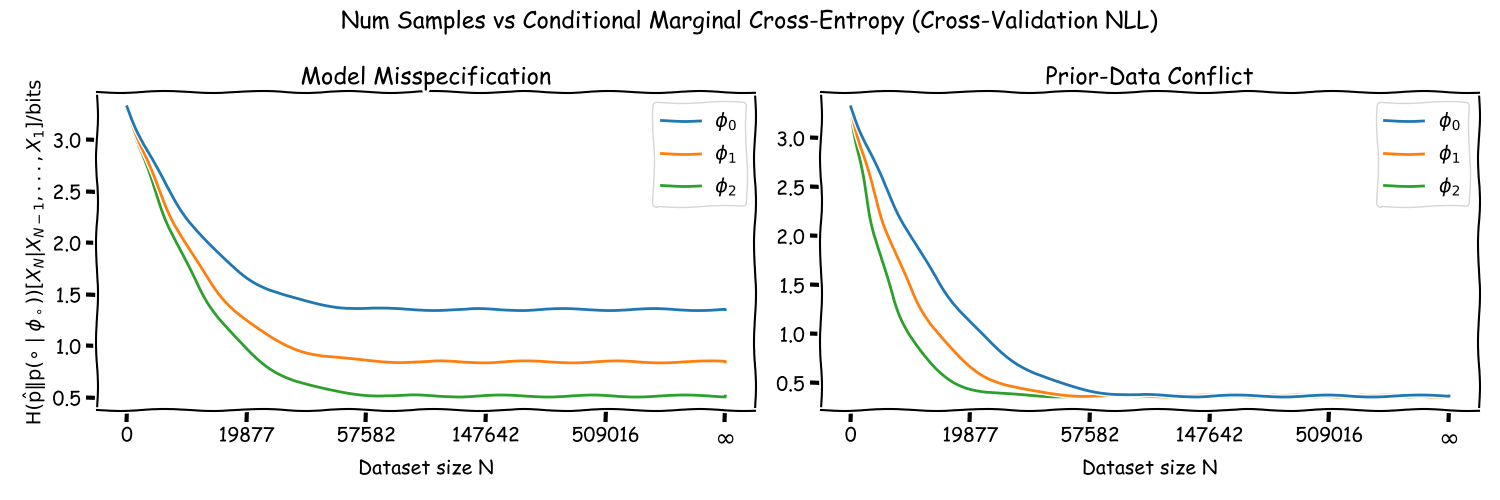
\includegraphics[width=\linewidth]{prior_conflict_and_model_misspecification_0.67.png}
      % \end{tikzpicture}  
    \end{backgroundbox}
    \begin{multicols}{2}
      \begin{theorybox}[title=Model Misspecification]
        \textbf{Model misspecification} occurs when the assumed model class does not contain the true data-generating process. In this case:
        \begin{itemize}
          \item Different models can have different levels of misspecification, leading to differences in performance.
          \item In the infinite data limit, the model with the lowest misspecification (i.e., the closest to the true data-generating process) will perform best.
        \end{itemize}
      \end{theorybox}
      \columnbreak
      \begin{theorybox}[title=Prior-Data Conflict]
        \textbf{Prior-data conflict} arises when the assumed prior distribution is inconsistent with the observed data. In this scenario:
        \begin{itemize}
        \item Models with priors that are more consistent with the observed data will perform better initially.
        \item The effect of prior-data conflict diminishes as the dataset size increases and the likelihood term dominates the prior term.
        \end{itemize}
      \end{theorybox}
    \end{multicols}
  }
\end{columns}
\end{document}
